\documentclass{article}
% PACKAGES
\usepackage[english]{babel}
\usepackage{graphicx} % Required for inserting images
\usepackage[most]{tcolorbox}
\usepackage{lmodern}
\usepackage{titlepic}
\usepackage{pdfpages}
\usepackage{tcolorbox}
\usepackage{amsmath}
\usepackage{pgfplots}
\usepackage{xcolor}
\usepackage{tikz}
\usepackage{color,soul}
\usepackage{enumerate}
\usepackage{enumitem}
\usepackage{cancel}
\usepackage{hyperref} 
\usepackage{tikzsymbols}
\usepackage{fontawesome5}
\usepackage[export]{adjustbox}
\usepackage{amssymb}
\usepackage{tikz,lipsum,lmodern}
\usepackage{booktabs}
\usepackage{tikz-3dplot}
\usepackage{circuitikz}

% COLOURS
\definecolor{Orchid}{RGB}{218, 112, 214}
\definecolor{snow}{rgb}{1.0, 0.98, 0.98}
\definecolor{mordantred19}{rgb}{0.68, 0.05, 0.0}
\definecolor{mistyrose}{rgb}{1.0, 0.89, 0.88}
\definecolor{nadeshikopink}{rgb}{0.96, 0.68, 0.78}
\definecolor{cadmiumgreen}{rgb}{0.0, 0.42, 0.24}
\definecolor{OliveGreen}{RGB}{85, 107, 47}
\definecolor{RoyalPurple}{RGB}{120, 81, 169}
\definecolor{NavyBlue}{RGB}{0, 0, 128}
\definecolor{CornflowerBlue}{RGB}{100, 149, 237}
\definecolor{Cerulean}{RGB}{0, 123, 167}
\definecolor{DarkOrchid}{RGB}{153, 50, 204}


\usetikzlibrary{calc}

\title{MCV4U - Calculus and Vectors [Chapter 8]}
\author{Kensukeken}
\date{May 20th, 2024}

\begin{document}
\maketitle

\tableofcontents
\newpage
\section{Unit 8 - Equations of Lines and Planes }
\subsection{Vector and Parametric Equations of a Line in $\mathbb{R}^2$}
To find the vector and/or parametric equation of a line in $\mathbb{R}$, we must be given two points on the line, or a point on the line a direction vector.\\
A direction vector is defined to be a vector $\vec{m}=\overrightarrow{(a,b)}$ that is parallel to (i.e colliear with) the line in question.

\subsubsection*{Example}
\begin{minipage}{0.45\textwidth}
    Sketch the line that has the point $(3,-2)$ on it, with the direction vector $\vec{m}=\overrightarrow{(4,-1)}$.
\end{minipage}%
\begin{minipage}{0.45\textwidth}
    \begin{center}
        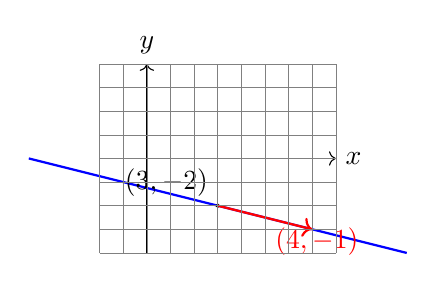
\begin{tikzpicture}[scale=0.3]
            % Define the point and the direction vector
            \coordinate (P) at (3, -2);
            \coordinate (Q) at ($(P) + (4, -1)$);

            % Draw the axes
            \draw[->] (-2,0) -- (8,0) node[right] {$x$};
            \draw[->] (0,-4) -- (0,4) node[above] {$y$};

            % Draw the line
            \draw[thick,blue] ($(P) - 2*(4,-1)$) -- ($(P) + 2*(4,-1)$);

            % Draw the point (3, -2)
            \filldraw (P) circle (2pt) node[above left] {$(3, -2)$};
            
            % Draw the direction vector
            \draw[->, red, thick] (P) -- (Q) node[midway, below right] {$(4, -1)$};

            % Add grid for reference
            \draw[step=1cm, gray, very thin] (-2, -4) grid (8, 4);
        \end{tikzpicture}
    \end{center}
\end{minipage}

\vspace{1cm}

\subsubsection*{Solution}
    \begin{align*}
        \vec{r} = \overrightarrow{(3,-2)} + t\overrightarrow{(4,-1)}, \quad t \in \mathbb{R} \\
        \vec{r} = \vec{r}_0 + t\vec{m}, \quad t \in \mathbb{R}
    \end{align*}
    Therefore, to travel from the origin to any point, we need to travel along the following journey:
    \[
        \vec{r} = \vec{r}_0 + t\vec{m}, \quad t \in \mathbb{R}
    \]
    This is the vector equation. \\
    In this example, the vector equation is $\vec{r} = \overrightarrow{(3,-2)} + t\overrightarrow{(4,-1)}, \quad t \in \mathbb{R}$, where $\overrightarrow{(3,-2)}$ is called the position vector, $\overrightarrow{(4,-1)}$ is called the direction vector, and $t$ is called a parameter.



\begin{tcolorbox}[colback=red!5!snow, colframe=red!50!white,
  colbacktitle=red!75!mistyrose]
The vector of a line in $\mathbb{R}^2$ is\\
\[
\vec{r} = \vec{r}_0 + t\vec{m}, t\in \mathbb{R}
\]
where 
\begin{itemize}
    \item  $\vec{r_0}$ is called the position vector 
    \item $\vec{m}$ is called the direction vector
    \item $t$ is called a parameter 
\end{itemize}
\end{tcolorbox}
\subsubsection{How to Develop the Parametric Equations }
If we are given the vector equation 
\[
    \vec{r}=\overrightarrow{(3,-2)}+t\overrightarrow{(4,-1)}, t \in \mathbb{R} 
\]
We can think of that as
\[
    \overrightarrow{(x,y)}=\overrightarrow{(3,-2)}+t\overrightarrow{(4,-1)}, t \in \mathbb{R}
\]

In turn, we can thunk of that as 
\[
    x=3+4t,y=-2-t,t\in \mathbb{R}
\]
These are the parametric equations of the line.
\subsubsection*{Example}
Determine the equation of a line is perpendicular to the line $\vec{r}=\overrightarrow{(5,-9)}+t\overrightarrow{(3,-5)}$ and that passes the point $(-5,-1)$
\subsubsection*{Solution}
\[
    \vec{r}=\overrightarrow{(5,-9)}+t\overrightarrow{(3,-5)}
\]
Perpendicular to a direction vector of $\overrightarrow{(3,-5)}$ is $\overrightarrow{(5,3)}$\\
Since the line for which we seek on equation contains the point $(-5,-1)$ as a position vector.\\
$\therefore$ the vector equation of the line being sought is $\vec{r}=\overrightarrow{(5,-1)}+t\overrightarrow{(5,3)}, t\in \mathbb{R}$


\subsection{Cartesian Equation of a Line in $\mathbb{R}^2$}
\begin{center}
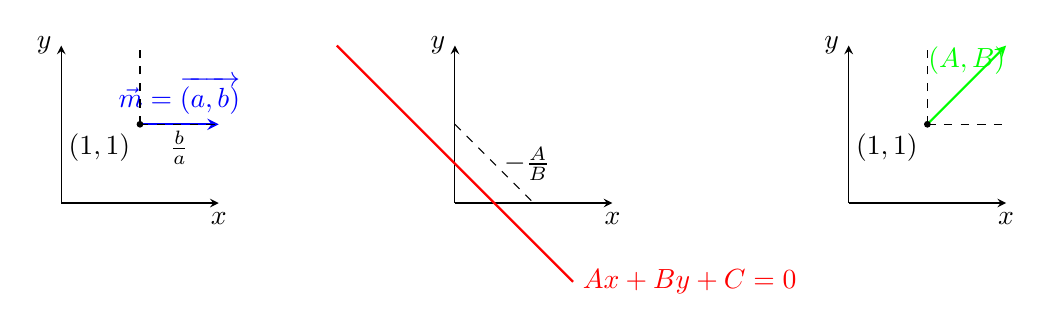
\begin{tikzpicture}[>=stealth]

    % Slope of a line
    \begin{scope}[shift={(0,0)}]
        \draw[->] (0,0) -- (2,0) node[below] {$x$};
        \draw[->] (0,0) -- (0,2) node[left] {$y$};
        \draw[thick, blue, ->] (1,1) -- (2,1) node[midway, above] {$\vec{m} = \overrightarrow{(a, b)}$};
        \filldraw (1,1) circle (1pt) node[below left] {$(1, 1)$};
        \draw[dashed] (1,1) -- (1,2);
        \draw[dashed] (1,1) -- (2,1);
        \node at (1.5, 0.7) {$\frac{b}{a}$};
    \end{scope}

    % Cartesian equation of a line
    \begin{scope}[shift={(5cm,0)}]
        \draw[->] (0,0) -- (2,0) node[below] {$x$};
        \draw[->] (0,0) -- (0,2) node[left] {$y$};
        \draw[thick, red] (-1.5,2) -- (1.5,-1);
        \node[right, red] at (1.5,-1) {$Ax + By + C = 0$};
        \draw[dashed] (0,1) -- (1,0);
        \node[right] at (0.5, 0.5) {$-\frac{A}{B}$};
    \end{scope}

    % Normal vector
    \begin{scope}[shift={(10cm,0)}]
        \draw[->] (0,0) -- (2,0) node[below] {$x$};
        \draw[->] (0,0) -- (0,2) node[left] {$y$};
        \draw[thick, green, ->] (1,1) -- (2,2) node[midway, above] {$(A, B)$};
        \filldraw (1,1) circle (1pt) node[below left] {$(1, 1)$};
        \draw[dashed] (1,1) -- (1,2);
        \draw[dashed] (1,1) -- (2,1);
    \end{scope}

\end{tikzpicture}
\end{center}

\begin{itemize}
    \item \textbf{Left:} If the slope of a line is $\frac{b}{a}$, then the direction vector is $\overrightarrow{(a,b)}$.
    \item \textbf{Middle:} If the Cartesian equation of a line is $Ax + By + C = 0$, then the slope of the line is $-\frac{A}{B}$.
    \item \textbf{Right:} If $Ax + By + C = 0$, then the normal vector is $(A,B)$.
\end{itemize}
\subsubsection*{Example}
Determine the equivalent vector and parametric equations of the line $y=\frac{3}{4}x+2$
\subsubsection*{Solution}
\begin{align*}
    y&=\frac{3}{4}x+2\\
    m&=\overrightarrow{(4,3)}\\
\end{align*}
a point on the line is $\overrightarrow{(0,2)}$\\
A point on the line is $\vec{r}_0 = \begin{pmatrix} 0 \\ 2 \end{pmatrix}$.

Therefore, a vector equation is $\vec{r} = \vec{r}_0 + t \vec{d}$, where $\vec{d} = \begin{pmatrix} 4 \\ 3 \end{pmatrix}$.

Parametric equations are:
$ x = 4t, \quad y = 2 + 3t, \quad t \in \mathbb{R}.$
\subsubsection*{Example }
The line segment joining $A(2,0)$ and $B(5,3)$ is the hypotenuse of a right triangle. The third vertex, C, lies on the line $\vec{r}=\overrightarrow{(3,1)}+t\overrightarrow{(1,-2)}$. Determine the coordinates of C(there might be more than one answer)

\subsubsection*{Solution}

\begin{minipage}{0.45\textwidth}
    \centering
    \resizebox{0.9\textwidth}{!}{%
        \begin{circuitikz}
        \tikzstyle{every node}=[font=\small]
        \node [font=\LARGE, color={rgb,255:red,255; green,0; blue,0}] at (13.5,16.75) {};
        \node [font=\LARGE] at (13.5,16.75) {};
        \draw [short] (5.25,9) -- (14,9);
        \draw [short] (7.5,14) -- (7.5,7);
        \draw [ color={rgb,255:red,0; green,51; blue,255}, short] (9.5,9) -- (9.5,12.5);
        \draw [ color={rgb,255:red,4; green,0; blue,255}, short] (9.25,12.5) -- (12.5,12.5);
        \draw [short] (12.5,12.5) -- (9,8.5);
        \draw [short] (9.5,12.25) -- (9.75,12.25);
        \draw [short] (9.75,12.5) -- (9.75,12.25);
        \draw [dashed] (7.5,14) -- (14,9);
        \node [font=\small] at (9.75,8.75) {A(2,0)};
        \node [font=\small] at (9.5,12.75) {C};
        \node [font=\small] at (12.5,12.75) {B(5,3)};
        \end{circuitikz}
    }%
\end{minipage}%
\begin{minipage}{0.55\textwidth}
    \begin{align*}
        &\overrightarrow{AC} \cdot \overrightarrow{BC} = 0 \\
        &\overrightarrow{AC} = \overrightarrow{(3+t-2,1-2t-0)} = \overrightarrow{(t+1,1-2t)} \\
        &\overrightarrow{(t+1,1-2t)} \cdot \overrightarrow{(t-2,-2-2t)} = 0 \\
        &(t+1)(t-2) + (1-2t)(-2-2t) = 0 \\
        &t^2 - t - 2 - 2 + 2t + 4t^2 = 0 \\
        &5t^2 + t - 4 = 0 \\
        &(5t-4)(t+1) = 0 \\
        &\boxed{t=\frac{4}{5} \text{ or } t=-1} \\
        &t=\frac{4}{5} \implies x=3+\frac{4}{5}=\frac{19}{5}, \\
        &\quad y=1-2\left(\frac{4}{5}\right)=-\frac{3}{5} \quad \therefore C \left(\frac{19}{5}, -\frac{3}{5}\right) \\
        &\text{or} \\
        &t=-1 \implies x=3-1=2, \quad y=1-2(1)=3 \quad \therefore C(2,3)
    \end{align*}
\end{minipage}



\newpage 
\subsection{Vector, Parametric and Symmetric Equations of a Line in $R^3$}
\subsubsection*{Example}
Determine the vector equation and parametric equations of a line that passes through the points $A(2,-3,4)$ and $B(8,1-9)$.
\subsubsection*{Solution}
\begin{align*}
\vec{m}=\overrightarrow{AB}&=\overrightarrow{(6,4,-13)}
\end{align*}
$\therefore$ a vector equation is a $\vec{r}=\overrightarrow{(2,-3,4)}+t\overrightarrow{(6,4,-13)}, t \in \mathbb{R}$ and parametric are:

\begin{align*}
    x&=2+6t\\
    y&=-3+4t\\
    z&=4-13t, t \in \mathbb{R}
\end{align*}

\subsubsection*{Example}
Show that the following two vector equations represents the same line.
\[
    L_1: \vec{r}=\overrightarrow{(3,1,0)}+s\overrightarrow{(-9,6,3)}, s \in \mathbb{R}
\]
\[
 L_2: \vec{r}=\overrightarrow{(-6,7,3)}+s\overrightarrow{(3,-2,-1)}, t \in \mathbb{R}
\]
\subsubsection*{Solution}
\underline{Part 1}
\[
\overrightarrow{m_1}=-3\overrightarrow{m_2}
\]

$\therefore$ lines are parallel collinear.\\\\
\underline{Part 2}\\
Next, show that a point on one line is on the other line.\\
We know that $(3,1,0)$ is a point on $L_1$ it is also on $L_2$.
\begin{align*}
    \text{let } 3&=-6+3t \implies 9=3t \implies \textcolor{red}{t=3}\\
    \text{let } 1&=7-2t \implies -6 =-2t \implies \textcolor{red}{t=3}\\
    \text{let } 0&=3-t \implies -3=-t \implies \textcolor{red}{t=3}
\end{align*}
Since the line are parallel and where a point $\therefore$ they are the same line.
\subsubsection*{Example}
Does the line $\vec{r}=\overrightarrow{(8,4-1)}+t\overrightarrow{(4,1,3)},t \in \mathbb{R}$ have a z-intercept?
\subsubsection*{Solution}
$z-int \implies x=0, y=0$\\
\[
    \implies 8+4t=0 \quad \text{ and } \quad 4+t=0
\]
We get $t=-2$ and $t=-4 \implies$ Not possible. Therefore, no z-intercepts 


\subsubsection{Symmetric Equation of a Line}
Suppose $\vec{r}=\overrightarrow{(x_0,y_0,z_0)}+t\overrightarrow{(a,b,c)}, t \in \mathbb{R}$ is the equation of a line in $\mathbb{R}^3$. Future, suppose that none of a a or b or c are zero. In other words, the components of the direction vector are all non-zero.\\

Then, the parametric equations of the line are:
\begin{align*}
    x&=x_0+ta\\
    y&=y_0+tb\\
    z&=z_0+tc, t \in \mathbb{R}
\end{align*}
Let's solve for t in each of these three parametric equations \\
\begin{align*}
    x=x_0+ta \quad y=y_0+td \quad z=z_0+tc\\
    x-x_0=ta \quad y-y_0=tb \quad z-z_0=tc\\
    \boxed{\frac{x-x_0}{a}=t} \quad \boxed{\frac{y-y_0}{b}=t} \quad \boxed{\frac{z-z_0}{c}=t}
\end{align*}

Now notice that in last line, t is equal to all of those quantities. That must mean that each of those quantities is equal to each other. In other words
\[
    \frac{x-x_0}{a}=\frac{y-y_0}{b}=\frac{z-z_0}{c}
\]

\begin{tcolorbox}[colback=red!5!snow, colframe=red!50!white,
  colbacktitle=red!75!mistyrose]
If the vector equation of a line is $\vec{r}=(x_0,y_0,z_0)+t\overrightarrow{(a,b,c)}, t \in \mathbb{R}$, then the symmetric equation of the line is:
\[
    \frac{x-x_0}{a}=\frac{y-y_0}{b}=\frac{z-z_0}{c}, a\neq 0, b \neq 0 , c \neq 0
\]

\end{tcolorbox}
\newpage 

\subsection{Vector and Parametric Equation of a Plane}
We know that a point on a line and a direction vector define a line in $\mathbb{R}^3$.\\
We also know that two non-zero, non-collinear vector span a plane in $\mathbb{R}^3$.\\
Putting these concepts together gives us this:

\begin{tcolorbox}[colback=red!5!snow, colframe=red!50!white,
  colbacktitle=red!75!mistyrose]
Two non-zero, non-collinear vectors and a point define a plane in $\mathbb{R}^3$  
\end{tcolorbox}
\subsubsection*{Example 1}
Given the plane with vector equation 
$\vec{r}=\overrightarrow{(1,5,-3)}+s\overrightarrow{(3,-4,6)}+t\overrightarrow{(4,5,-8)}$ and parametric equations $x=1+3s+4t, y=5-4s+5t$ and $z=-3+6s-8$, determine whether the point (11,2,3) is on the plane.
\subsubsection*{Solution}
Substitute \(x = 11\), \(y = 2\), and \(z = 3\) into the parametric equations:
\[
\begin{cases}
11 = 1 + 3s + 4t \\
2 = 5 - 4s + 5t \\
3 = -3 + 6s - 8t
\end{cases}
\]

Simplify each equation:
\[
\begin{cases}
10 = 3s + 4t \quad \text{(1)} \\
-3 = -4s + 5t \quad \text{(2)} \\
6 = 6s - 8t \quad \text{(3)}
\end{cases}
\]

Solve equations (1) and (2):
\[
4 \times (3s + 4t) = 40 \implies 12s + 16t = 40
\]
\[
3 \times (4s - 5t) = 9 \implies 12s - 15t = 9
\]
Subtract:
\[
31t = 31 \implies t = 1
\]
Substitute \(t = 1\) into (1):
\[
3s + 4(1) = 10 \implies 3s + 4 = 10 \implies 3s = 6 \implies s = 2
\]
Verify with (3):
\[
6(2) - 8(1) = 12 - 8 = 4 \neq 6
\]

Therefore, the point \((11, 2, 3)\) is not on the plane.


In summary, to determine whether a given point is on a given plane when the plane is written in vector form or in parametric form, we need to get the plane into parametric form. Then, we can set the x-coordinate of the point in question equal to the parametric expression for x and we set the y-coordinate of the point in question equal to the parametric expression for y. Then, we usually use substitution or elimination to solve for the parameters (usually s and t). Then, we plug those parameter values into the parametric expression for z and see if we get the required value of the z-coordinate.

\subsubsection{More Information About Planes}
One and only one plane can be determined if we are given any of the following:
\begin{itemize}
    \item a line and a point not on the line
    \item three non-collinear points (three points not on a line)
    \item two intersecting lines
    \item two parallel and non-coincident lines
\end{itemize}
\subsubsection*{Example 2}
Determine a vector equation and parametric equations for the plane containing the points \(A (6, 2, 1)\), \(B (9, -4, 2)\), and \(C (-1, -2, -3)\).

\subsubsection*{Solution}
\begin{align*}
    &\overrightarrow{AB} = \langle 9-6, -4-2, 2-1 \rangle = \langle 3, -6, 1 \rangle \\
    &\overrightarrow{AC} = \langle -1-6, -2-2, -3-1 \rangle = \langle -7, -4, -4 \rangle \\
    &\vec{n} = \overrightarrow{AB} \times \overrightarrow{AC} = \begin{vmatrix}
        \mathbf{i} & \mathbf{j} & \mathbf{k} \\
        3 & -6 & 1 \\
        -7 & -4 & -4
    \end{vmatrix} = \mathbf{i}(24 + 4) - \mathbf{j}(-12 + 7) + \mathbf{k}(-12 + 42) = \langle 28, 5, 30 \rangle \\
    &\text{Vector equation:} \quad \vec{r} = \begin{pmatrix} 6 \\ 2 \\ 1 \end{pmatrix} + s \begin{pmatrix} 3 \\ -6 \\ 1 \end{pmatrix} + t \begin{pmatrix} -7 \\ -4 \\ -4 \end{pmatrix} \\
    &\text{Parametric equations:} \quad \begin{cases}
    x = 6 + 3s - 7t \\
    y = 2 - 6s - 4t \\
    z = 1 + s - 4t
    \end{cases}
\end{align*}

\subsubsection*{Example 3}
Given the plane with parametric equations \(x=6+3s+7t\), \(y=2-6s+4t\), \(z=1+s+4t\), \(s, t \in \mathbb{R}\), determine the point where this plane intersects the x-axis.

\subsubsection*{Solution}
For the plane to intersect the x-axis, \(y = 0\) and \(z = 0\):
\begin{align*}
    &2 - 6s + 4t = 0 \quad \text{(Equation 1)} \\
    &1 + s + 4t = 0 \quad \text{(Equation 2)}
\end{align*}
From Equation 2:
\[
s = -1 - 4t
\]
Substitute \(s = -1 - 4t\) into Equation 1:
\[
2 - 6(-1 - 4t) + 4t = 0 \implies 2 + 6 + 24t + 4t = 0 \implies 8 + 28t = 0 \implies t = -\frac{2}{7}
\]
Substitute \(t = -\frac{2}{7}\) back into \(s = -1 - 4t\):
\[
s = -1 - 4\left(-\frac{2}{7}\right) = -1 + \frac{8}{7} = -\frac{7}{7} + \frac{8}{7} = \frac{1}{7}
\]
Find the corresponding \(x\) value:
\[
x = 6 + 3\left(\frac{1}{7}\right) + 7\left(-\frac{2}{7}\right) = 6 + \frac{3}{7} - 2 = 6 - 2 + \frac{3}{7} = 4 + \frac{3}{7} = \frac{28}{7} + \frac{3}{7} = \frac{31}{7}
\]
Therefore, the point of intersection is:
\[
\left( \frac{31}{7}, 0, 0 \right)
\]

\subsection{Cartesian Equation of a Plane (Aka Scalar Equation of a Plane)}

\begin{tcolorbox}[colback=red!5!snow, colframe=red!50!white,
  colbacktitle=red!75!mistyrose]
The Cartesian (or scalar) equation of a plane in $\mathbb{R}^3$ is of the form $Ax+Bx+Cz+D=0$. \\
The vector $\overrightarrow{(A,B,C)}$ is a normal vector (perpendicular to all of the vectors in the plane)
\end{tcolorbox}  
\subsubsection{Angle Between Two Planes}
\begin{tcolorbox}[colback=red!5!snow, colframe=red!50!white,
  colbacktitle=red!75!mistyrose]
Two angle between two planes is equal to the angle between the normal vectors of the two planes
  
\end{tcolorbox}  
\end{document}